\begin{frame}{Avant la plongée}
\centering%
%\includegraphics<1>[width=2cm]{Sorties_2024-2025}%
\includegraphics<1>[width=2cm]{Agenda_AMP}%
\begin{block}<only@1>{}
\begin{itemize}
\item Vérification du niveau pour la plongée;
\item inscription sur le site;
\item pré-paiement suivant la plongée.
\end{itemize}
\end{block}%
\includegraphics<1>[width=2cm]{inscription2}%
%\includegraphics<2>[width=\textwidth]{Sorties_2024-2025}%
\includegraphics<2>[height=6.5cm]{Agenda_AMP}%
\only<3>{\juxt[0.3]{\includegraphics[width=\textwidth]{equipement}}{%
\begin{block}{Préparation du sac}
\begin{itemize}
\item Maillot, serviette, moyens de paiement, crème solaire, vêtements de rechange\dots;
\item équipement: combinaison, masque, détendeur, gilet, palmes, bouteille;
\item paperasse: \Emph{licence}, \Emph{certificat médical}, \Emph{carte niveau}, carnet de plongée;
\item de quoi manger (sandwich/salade/\dots, eau).
\end{itemize}
\end{block}}}%
\includegraphics<4>[width=3cm]{covoit}%
\begin{block}<only@4>{Covoiturage}
Lieu de rendez-vous, prévoir une place dans une voiture ou
proposer des places dans sa voiture
\end{block}%
\end{frame}

\begin{frame}{Sur le lieu de la plongée}
\juxt[0.7]{%
\begin{block}{Papiers!}
Présenter ses papiers au DP
\end{block}
\begin{block}{Préparer ses affaires}
\begin{itemize}
\item Vérification et gréage de son bloc.
\item Bouteille fermée et allongée ou accrochée sur le bateau.
\end{itemize}
\end{block}
\begin{block}{Embarquer}
\begin{itemize}
\item Bloc et affaires fixés sur le bateau, rien ne traine.
\item Combinaison suivant DP/GP.
\end{itemize}
\end{block}}{%
\null\hfill\papieren{\textwidth}\hfill\null\\
\includegraphics[width=\textwidth]{blocs}
}
\end{frame}

\begin{frame}{Sur le trajet en mer}
\juxt{%
\begin{block}{}
\begin{itemize}[<+->]
\item On ne gêne pas;
\item on écoute les consignes (pilote, directeur de plongée, son guide);
\item on s'équipe (consignes guide);
\item mise à l'eau (bascule arrière, saut droit) \Emph{après} son guide.
\end{itemize}
\end{block}}
{%
\includegraphics<1-2>[width=\textwidth]{bateau}%
\includegraphics<3>[width=\textwidth]{sequipe}%
\includegraphics<4>[width=\textwidth]{saut_droit}%
}
\end{frame}

\begin{frame}{Dans l'eau}
\only<1-3>{\null\hfill\includegraphics[width=4cm]{descente}\hfill\includegraphics[width=4cm]{oreilles}\hfill\null}%
\begin{block}<only@1-3>{L'immersion}
\begin{itemize}[<+->]
\item Sur signe du guide, phoque ou canard;
\item descente au-dessus du guide;
\item attention aux \Emph{oreilles}, équilibrage tout le long.
\end{itemize}
\end{block}%
\only<4-9>{%
\juxt[0.6]{\begin{block}{La balade}
\begin{itemize}[<+->]
\item Proche du guide, même profondeur;
\item suis ses instructions;
\item on communique, on donne sa consommation d'air;
\item on communique, si froid, si essouflement, si quoi que ce soit;
\item on profite.
\item<+-| alert@+> Si on perd sa palanquée
\end{itemize}
\end{block}}{\includegraphics[width=\textwidth]{palanquee}}}
\only<10>{\null\hfill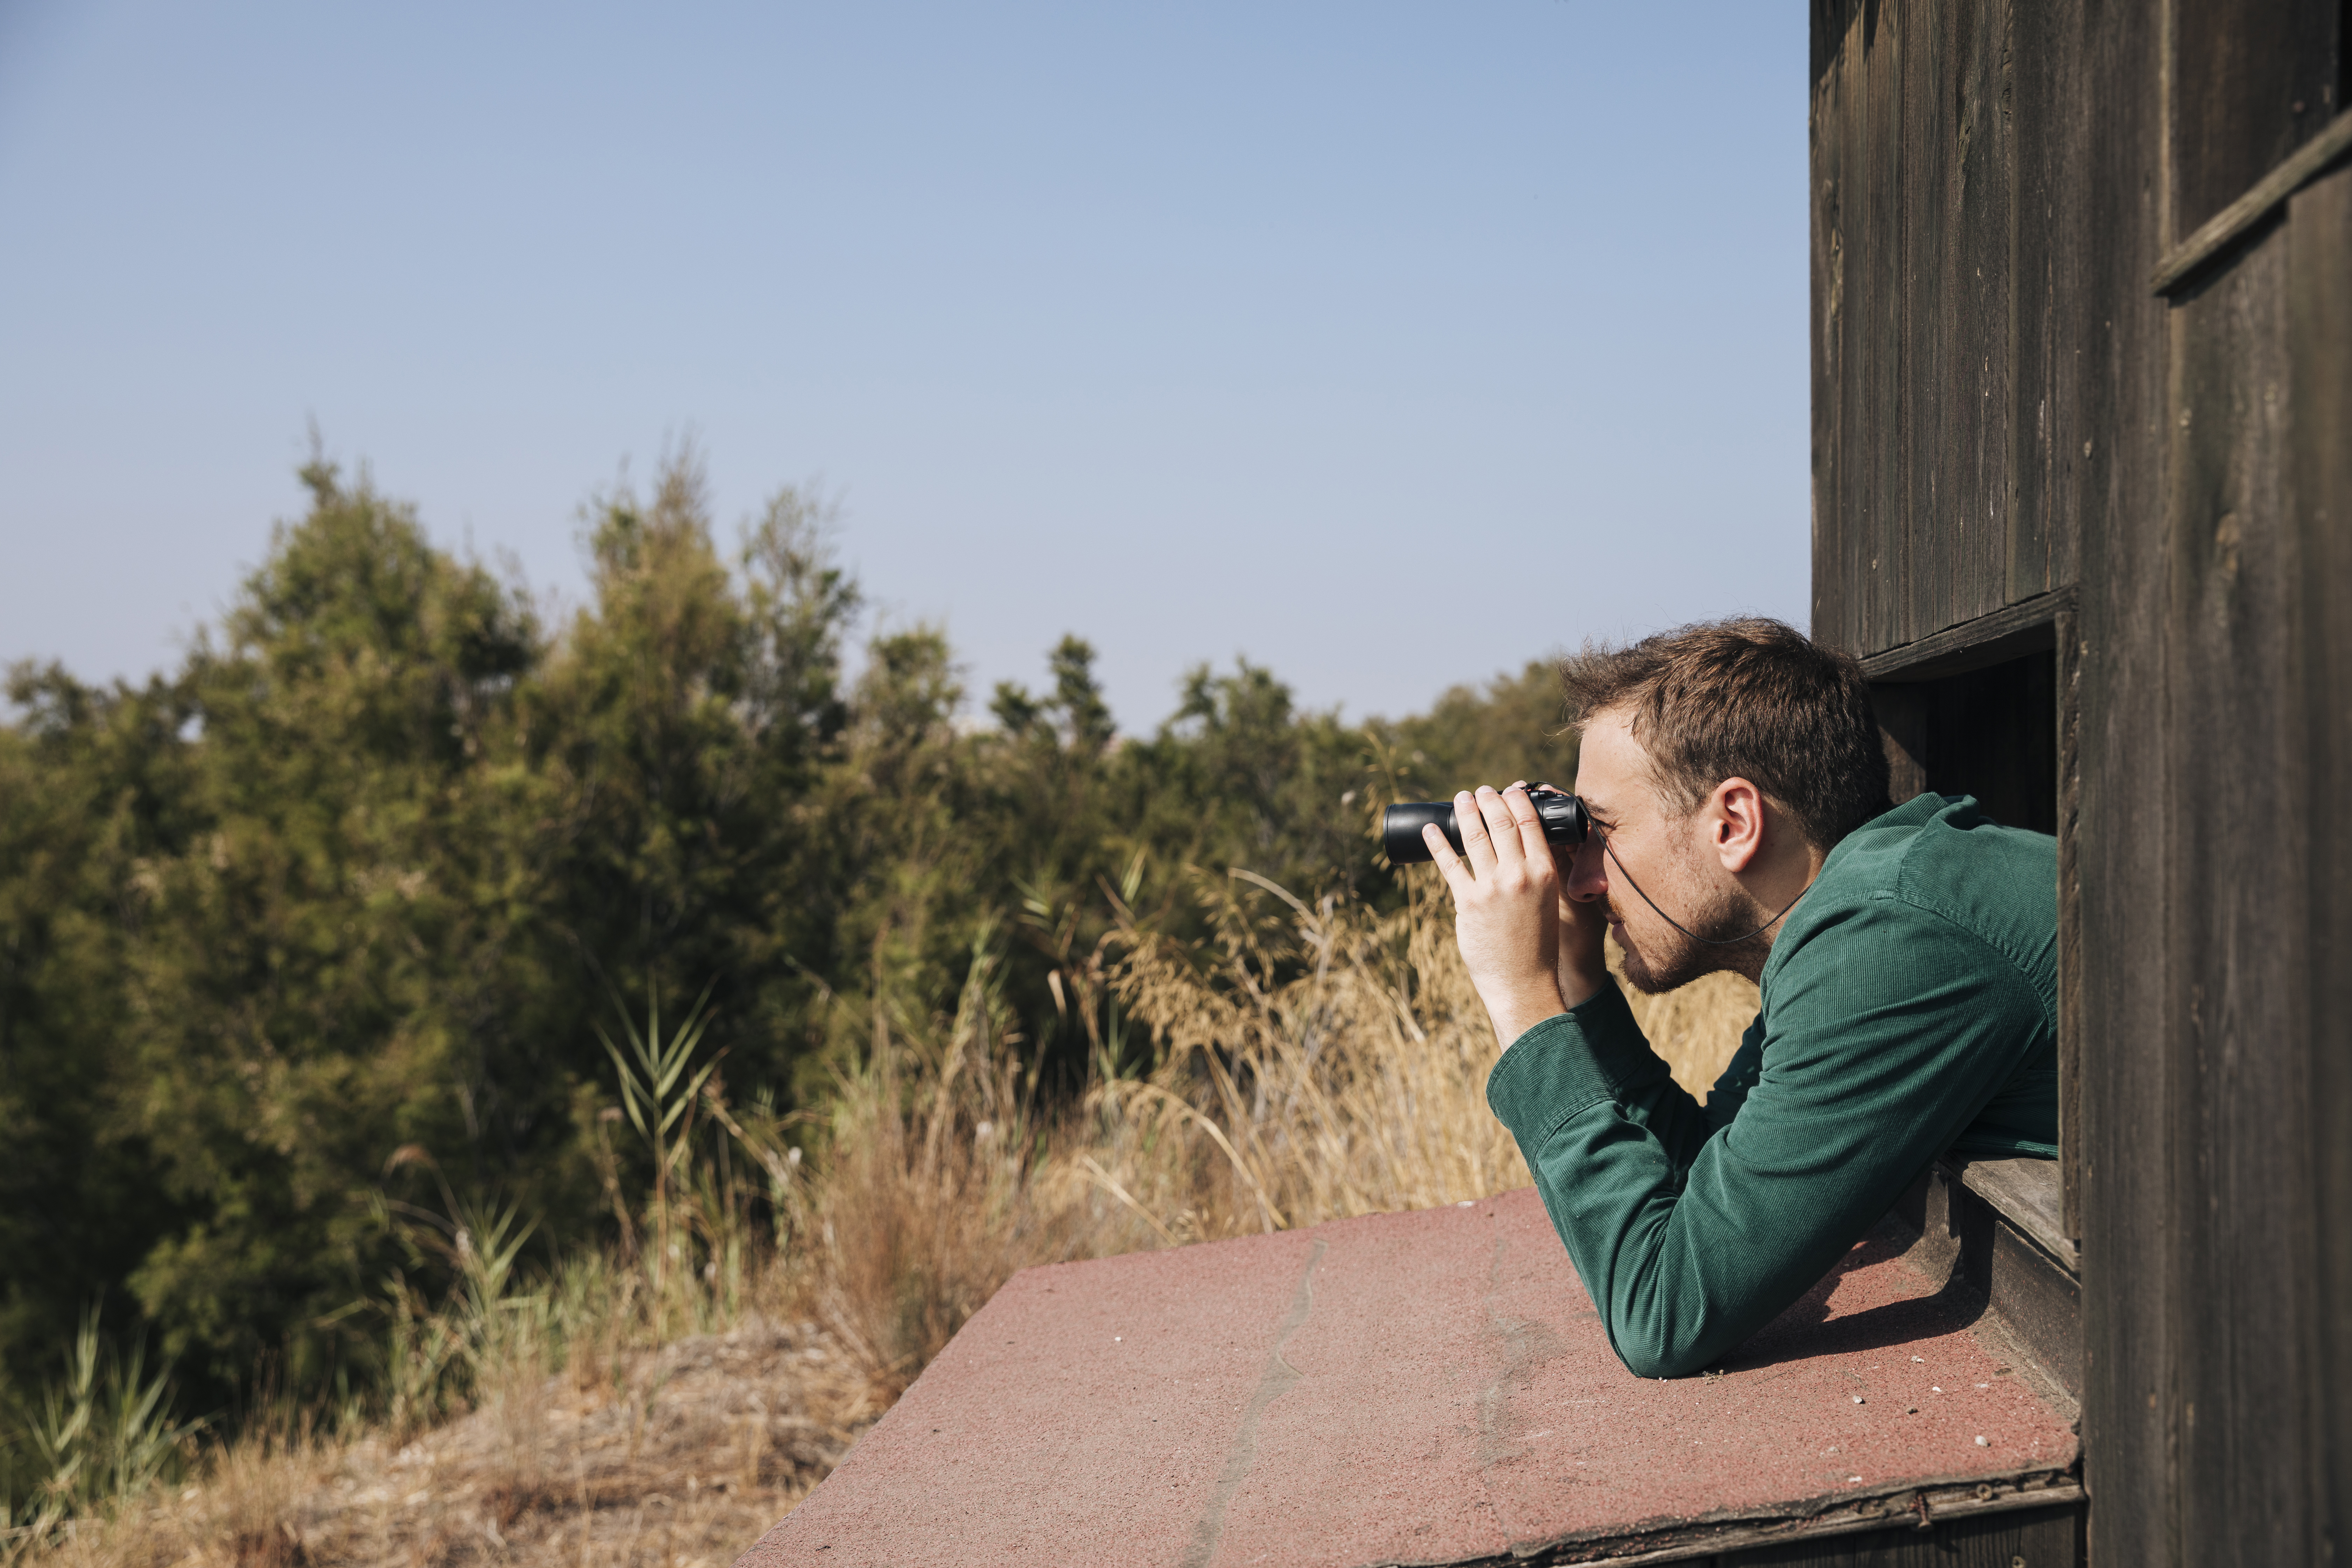
\includegraphics[width=3cm]{recherche}\hfill\includegraphics[width=3cm]{remontee}\hfill\null}%
\begin{block}<only@10>{}
\begin{itemize}
\item On cherche environ 1~minute, on remonte de quelques
  mètres, on cherche les bulles,
\item on remonte \EMPH{doucement}, en \EMPH{soufflant}, et on se retrouve à la
  surface.
\end{itemize}
\end{block}%
\begin{block}<only@11->{La remontée}
\begin{itemize}[<+(7)->]
\item Sur signe du guide;
\item juste sous le guide;
\item gestion du gilet;
\item on souffle;
\item on n'équilibre pas ses oreilles;
\item palier à 3 mètres possible;
\item tour d'horizon à l'approche de la surface;
\item gonfle le gilet à la surface;
\item remontée sur le bateau sur indication du guide,
  masque sur le visage et détendeur en bouche. On ne traîne pas sous l'échelle.%
\end{itemize}%
\end{block}%
\only<11->{%
\vskip -1cm\makebox[0pt][l]{\raisebox{1.8cm}[0pt][0pt]{\rule{0.6\textwidth}{0pt}%
\includegraphics<11-12>[width=4cm]{up}%
\includegraphics<13>[width=3cm]{gilet}%
\includegraphics<14-17>[width=4cm]{souffle}%
\includegraphics<18>[width=4cm]{surface}%
\includegraphics<19>[width=4cm]{echelle}%
}}}%
\end{frame}

\begin{frame}{Le retour}
\null\hfill\includegraphics[height=3cm]{blocs}\hfill\includegraphics[height=3cm]{hydrate}\hfill\null%
\begin{block}{}
\begin{itemize}[<+->]
\item Déséquipe, matériel fixé, rien ne traîne;
\item on se sèche;
\item on s'hydrate.
\end{itemize}
\end{block}
\end{frame}

\begin{frame}{Après la plongée}
\begin{block}{}
\begin{itemize}
\item<1-> \twemoji{woman in lotus position: medium skin tone}Pas d'efforts;
\item<.-> pas d'apnée;
\item<.-> pas d'altitude (montagne, avion);
\item<2-> on continue de s'hydrater;
\item<3-> on rince si possible le matériel;
\item<3-> on complète son carnet de plongée;
\item<3-> on range;
\item<4> on rentre;
\item<4> on rince le matériel si non rincé, on l'étend;
\item<4> on est heureux(se).
\end{itemize}
\end{block}
\makebox[0pt][l]{\raisebox{4.5cm}[0pt][0pt]{\rule{0.6\textwidth}{0pt}\includegraphics[width=3cm]{zen}}}%
\only<2->{\makebox[0pt][l]{\raisebox{1cm}[0pt][0pt]{\rule{0.72\textwidth}{0pt}\includegraphics[width=2.7cm]{hydrate}}}}%
\only<3->{\makebox[0pt][l]{\raisebox{2cm}[0pt][0pt]{\rule{0.62\textwidth}{0pt}\includegraphics[width=2.5cm]{carnet_plongee}}}}%
\only<4>{\makebox[0pt][l]{\raisebox{2.1cm}[0pt][0pt]{\rule{0.61\textwidth}{0pt}
\includegraphics[width=4cm]{bonheur}\makebox[0pt][r]{\tiny\textcolor{violet}{Image de Freepik}}}}}%
\end{frame}
